\documentclass[12pt,a4paper]{article}
\usepackage[utf8]{inputenc}
\usepackage{amsmath, amssymb}
\usepackage{graphicx}
\usepackage{geometry}
\usepackage{float}
\usepackage{booktabs}
\usepackage{circuitikz}
\usepackage{caption}
\usepackage{subcaption}
\usepackage{enumitem}
\setlist{itemsep=2pt, parsep=1pt, topsep=3pt}
\geometry{a4paper, margin=1in}

\title{\textbf{Characteristics of MOSFET}}
\author{Yamulapalli Nandu Navadeep \\ Roll Number: IMS24267}
\date{Date of Experiment: 30/09/2026 \\ Date of Submission: 15/10/2026}

\begin{document}

\maketitle

\section{Name of the Experiment}
Characteristics of an N-Channel Enhancement MOSFET.

\section{Aim of the Experiment}
\begin{enumerate}
    \item To study the transfer characteristics ($I_D$ versus $V_{GS}$) of an n-channel enhancement mode MOSFET and determine its threshold voltage ($V_T$).
    \item To study the drain (output) characteristics ($I_D$ versus $V_{DS}$) of the MOSFET at constant gate voltages and calculate the transconductance ($g_m$) and dynamic drain resistance ($r_d$).
\end{enumerate}

\section{Theory}
A Metal Oxide Semiconductor Field Effect Transistor (MOSFET) is a three-terminal semiconductor device widely used for switching and signal amplification. Unlike a Bipolar Junction Transistor (BJT), which is a current-controlled device requiring a continuous base current, a MOSFET is a voltage-controlled device where the current between the drain and source is modulated by the electric field created by the gate voltage.

The three primary terminals of a MOSFET are:
\begin{itemize}
    \item \textbf{Source (S):} The terminal through which majority charge carriers enter the conducting channel.
    \item \textbf{Drain (D):} The terminal through which majority charge carriers leave the channel.
    \item \textbf{Gate (G):} The control electrode that regulates the conductivity of the channel.
\end{itemize}

In a MOSFET, the gate electrode is electrically isolated from the semiconductor substrate by an extremely thin dielectric layer of silicon dioxide ($\text{SiO}_2$). Because of this insulation, the gate leakage current is practically zero, providing the MOSFET with an exceptionally high input impedance (often exceeding $10^{12}\ \Omega$).

\subsection{Enhancement Mode Operation and Channel Inversion}
In an n-channel enhancement MOSFET, the source and drain are heavily doped n-type regions diffused into a p-type silicon substrate. Under zero gate bias ($V_{GS} = 0$), two back-to-back p-n junctions exist between the drain and source, preventing current flow regardless of the applied drain voltage. Thus, the device is normally `OFF'.

When a positive gate-to-source voltage ($V_{GS} > 0$) is applied:
\begin{enumerate}
    \item The positive electric field repels holes (majority carriers in the p-substrate) away from the oxide-semiconductor interface, forming a depletion region of immobile negative acceptor ions.
    \item As $V_{GS}$ increases, minority electrons in the p-substrate are attracted towards the surface immediately beneath the gate oxide.
    \item When $V_{GS}$ exceeds a critical threshold voltage ($V_T$), the surface concentration of electrons exceeds the hole concentration. This layer of induced electrons forms an n-type conducting bridge between the drain and source, known as the \textbf{inversion layer} or n-channel.
\end{enumerate}

\subsection{Operating Regions}
Depending on the biasing voltages $V_{GS}$ and $V_{DS}$, the MOSFET operates in three primary functional regimes:
\begin{enumerate}
    \item \textbf{Cut-off Region ($V_{GS} < V_T$):}
    The gate voltage is insufficient to induce the inversion channel. The drain current is virtually zero ($I_D \approx 0$), and the transistor acts as an open switch.
    
    \item \textbf{Ohmic / Linear Region ($V_{GS} > V_T$ and $V_{DS} < V_{DSat}$):}
    Here, the drain-to-source voltage is less than the saturation voltage, where $V_{DSat} = V_{GS} - V_T$. A continuous conductive channel extends from source to drain. The channel behaves like a voltage-controlled linear resistor whose resistance is modulated by $V_{GS}$. The drain current is expressed as:
    \begin{equation}
        I_D = \mu_n C_{ox} \frac{W}{L} \left[ (V_{GS} - V_T)V_{DS} - \frac{V_{DS}^2}{2} \right]
    \end{equation}
    For very small values of $V_{DS}$ ($V_{DS} \ll V_{GS} - V_T$), the quadratic term can be neglected, yielding:
    \begin{equation}
        I_D \approx \mu_n C_{ox} \frac{W}{L} (V_{GS} - V_T) V_{DS}
    \end{equation}
    where $\mu_n$ is electron mobility, $C_{ox}$ is oxide capacitance per unit area, $W$ is channel width, and $L$ is channel length.
    
    \item \textbf{Saturation Region ($V_{GS} > V_T$ and $V_{DS} \ge V_{GS} - V_T$):}
    As $V_{DS}$ increases, the effective voltage across the oxide near the drain end, given by $V_{GD} = V_{GS} - V_{DS}$, decreases. When $V_{DS} = V_{DSat} = V_{GS} - V_T$, the channel depth at the drain end drops to zero; this condition is known as \textbf{pinch-off}. Beyond pinch-off, any further increase in $V_{DS}$ does not widen the channel; instead, electrons are swept across the depleted space-charge region by the strong drain electric field. The drain current becomes virtually independent of $V_{DS}$ and saturates at:
    \begin{equation}
        I_D = \frac{1}{2} \mu_n C_{ox} \frac{W}{L} (V_{GS} - V_T)^2 = K (V_{GS} - V_T)^2
    \end{equation}
    where $K = \frac{1}{2}\mu_n C_{ox} (W/L)$ is the conduction parameter. Taking the square root gives:
    \begin{equation}
        \sqrt{I_D} = \sqrt{K} (V_{GS} - V_T)
    \end{equation}
    This linear relationship allows precise determination of the threshold voltage $V_T$ by identifying the intercept on the horizontal axis.
\end{enumerate}

\subsection{Key Parameters}
\begin{itemize}
    \item \textbf{Threshold Voltage ($V_T$):} The minimum gate-to-source voltage required to induce the inversion layer and initiate drain current flow.
    \item \textbf{Transconductance ($g_m$):} Measures the control sensitivity of the gate voltage over the drain current at a constant drain voltage:
    \begin{equation}
        g_m = \left( \frac{\Delta I_D}{\Delta V_{GS}} \right)_{V_{DS} = \text{const}}
    \end{equation}
    \item \textbf{Dynamic Drain Resistance ($r_d$):} The inverse slope of the drain characteristics curve at a constant gate voltage:
    \begin{equation}
        r_d = \left( \frac{\Delta V_{DS}}{\Delta I_D} \right)_{V_{GS} = \text{const}}
    \end{equation}
\end{itemize}

\section{Procedure}

\subsection{Drain (Output) Characteristics}
\begin{enumerate}
    \item Assemble the circuit on the breadboard as shown in the circuit diagram, with gate protection resistor $R_G = 100\text{ k}\Omega$ and drain resistor $R_D = 1\text{ k}\Omega$.
    \item Adjust the gate power supply $V_{GG}$ until the gate-to-source voltmeter reads a constant value of $V_{GS} = 3.5\text{ V}$. Keep this gate voltage fixed.
    \item Gradually increase the drain power supply $V_{DD}$ so that $V_{DS}$ increases in steps from $0\text{ V}$ up to $17\text{ V}$.
    \item At each step of $V_{DS}$, record the corresponding drain current $I_D$ indicated by the milliammeter.
    \item Reduce $V_{DD}$ back to zero, set $V_{GS}$ to $3.6\text{ V}$, and repeat the complete sweep of $V_{DS}$ from $0\text{ V}$ to $17\text{ V}$.
    \item Repeat the entire process once more for $V_{GS} = 3.7\text{ V}$.
    \item Tabulate all recorded values and plot $I_D$ versus $V_{DS}$ for each constant value of $V_{GS}$.
\end{enumerate}

\subsection{Transfer Characteristics}
\begin{enumerate}
    \item Using the same circuit configuration, adjust the drain power supply $V_{DD}$ to maintain a constant drain-to-source voltage of $V_{DS} = 10\text{ V}$ (ensuring operation in the saturation region).
    \item Set the gate voltage $V_{GS}$ initially to $3.0\text{ V}$ using $V_{GG}$.
    \item Increase $V_{GS}$ in systematic steps of $0.1\text{ V}$ up to $3.7\text{ V}$.
    \item For every step of $V_{GS}$, read and note the resulting drain current $I_D$ on the milliammeter.
    \item Identify the onset voltage where drain current starts to flow ($V_T$).
    \item Plot $I_D$ versus $V_{GS}$ as well as $\sqrt{I_D}$ versus $V_{GS}$ to evaluate $V_T$ and the transconductance $g_m$.
\end{enumerate}

\section{Circuit Diagram}
\begin{figure}[H]
\centering
\begin{circuitikz}[scale=1, transform shape]
    % MOSFET
    \draw (0,0) node[nigfete] (M) {};
    \node[right] at (M.D) {D};
    \node[left] at (M.G) {G};
    \node[right] at (M.S) {S};

    % Source to Ground
    \draw (M.S) to[short] (0,-1) node[ground] (gnd) {};

    % Gate connection
    \draw (M.G) to[short] (-1.5,0) coordinate (G_node)
          to[R, l_={$R_G = 100\text{ k}\Omega$}] (-4,0)
          to[battery2, l_=$V_{GG}$] (-4,-1) node[ground] {};

    % Voltmeter V_GS across Gate and Source
    \draw (G_node) to[short, *-] (-1.5,-0.3)
          to[rmeter, t=V, l_=$V_{GS}$] (-1.5,-1) node[ground] {};

    % Drain connection
    \draw (M.D) to[short] (0,1.2) coordinate (D_node)
          to[R, l={$R_D = 1\text{ k}\Omega$}] (0,2.5)
          to[rmeter, t=mA, l=$I_D$] (2.5,2.5)
          to[battery2, l=$V_{DD}$] (2.5,0)
          to[short] (2.5,-1) node[ground] {};

    % Voltmeter V_DS across Drain and Source
    \draw (D_node) to[short, *-] (1.3,1.2)
          to[rmeter, t=V, l=$V_{DS}$] (1.3,-0.3)
          to[short] (1.3,-1) node[ground] {};

\end{circuitikz}
\caption{Experimental circuit diagram for investigating MOSFET characteristics}
\end{figure}

\section{Tabular Column}

\begin{table}[H]
\centering
\begin{minipage}[t]{0.52\textwidth}
\centering
\caption{Drain Characteristics ($I_D$ vs $V_{DS}$)}
\begin{tabular}{|c|c|c|c|}
\hline
\textbf{$V_{DS}$} & \multicolumn{3}{c|}{\textbf{Drain Current $I_D$ (mA)}} \\
\cline{2-4}
\textbf{(V)} & \textbf{$3.5\text{ V}$} & \textbf{$3.6\text{ V}$} & \textbf{$3.7\text{ V}$} \\
\hline
0.0 & 0 & 0 & 0 \\
0.2 & 0 & 0 & 0 \\
0.5 & 1 & 1 & 1 \\
1.0 & 2 & 1 & 1 \\
2.0 & 2 & 2 & 2 \\
3.0 & 3 & 3 & 3 \\
4.0 & 3 & 4 & 4 \\
5.0 & 3 & 5 & 5 \\
6.0 & 3 & 6 & 6 \\
7.0 & 3 & 7 & 7 \\
8.0 & 3 & 7 & 8 \\
9.0 & 3 & 7 & 9 \\
10.0 & 3 & 7 & 10 \\
11.0 & 3 & 7 & 11 \\
12.0 & 3 & 7 & 12 \\
13.0 & 3 & 7 & 14 \\
14.0 & 3 & 7 & 15 \\
15.0 & 3 & 7 & 16 \\
16.0 & 3 & 7 & 16 \\
17.0 & 3 & 7 & 16 \\
\hline
\end{tabular}
\end{minipage}
\hfill
\begin{minipage}[t]{0.45\textwidth}
\centering
\caption{Transfer Characteristics ($V_{DS} = 10\text{ V}$)}
\begin{tabular}{|c|c|c|}
\hline
\textbf{$V_{GS}$ (V)} & \textbf{$I_D$ (mA)} & \textbf{$\sqrt{I_D}\ (\text{mA}^{1/2})$} \\
\hline
3.0 & 0 & 0.00 \\
3.1 & 0 & 0.00 \\
3.2 & 0 & 0.00 \\
3.3 & 1 & 1.00 \\
3.4 & 1 & 1.00 \\
3.5 & 3 & 1.73 \\
3.6 & 8 & 2.83 \\
3.7 & 10 & 3.16 \\
\hline
\end{tabular}
\end{minipage}
\end{table}

\section{Calculations}

\subsection{Threshold Voltage ($V_T$)}
From the transfer characteristics observations recorded at $V_{DS} = 10\text{ V}$:
\begin{itemize}
    \item For $V_{GS} \le 3.2\text{ V}$, the channel remains non-conductive and $I_D = 0\text{ mA}$.
    \item Conduction initiates at $V_{GS} = 3.3\text{ V}$ with $I_D = 1\text{ mA}$.
\end{itemize}
In the saturation regime, the relationship between drain current and gate voltage is:
\begin{equation}
    \sqrt{I_D} = \sqrt{K} (V_{GS} - V_T)
\end{equation}
A linear fit performed over the active conduction region ($V_{GS}$ between $3.2\text{ V}$ and $3.7\text{ V}$) yields:
\begin{equation}
    \text{Slope } \sqrt{K} \approx 6.29\text{ mA}^{1/2}/\text{V}, \quad \text{Intercept } C \approx -20.09\text{ mA}^{1/2}
\end{equation}
Setting $\sqrt{I_D} = 0$ gives the threshold voltage:
\begin{equation}
    V_T = -\frac{C}{\sqrt{K}} = \frac{20.09}{6.29} \approx 3.19\text{ V} \approx 3.20\text{ V}
\end{equation}

\subsection{Transconductance ($g_m$)}
Transconductance is calculated from the steep slope of the transfer characteristic curve at $V_{DS} = 10\text{ V}$. Taking the data points in the active region between $V_{GS1} = 3.5\text{ V}$ ($I_{D1} = 3\text{ mA}$) and $V_{GS2} = 3.7\text{ V}$ ($I_{D2} = 10\text{ mA}$):
\begin{equation}
    g_m = \frac{\Delta I_D}{\Delta V_{GS}} = \frac{I_{D2} - I_{D1}}{V_{GS2} - V_{GS1}} = \frac{10\text{ mA} - 3\text{ mA}}{3.7\text{ V} - 3.5\text{ V}} = \frac{7\text{ mA}}{0.2\text{ V}} = 35.0\text{ mS}
\end{equation}
In standard SI units:
\begin{equation}
    g_m = 35.0 \times 10^{-3}\ \Omega^{-1} = 3.50 \times 10^{-2}\text{ S}
\end{equation}

\subsection{Dynamic Drain Resistance ($r_d$)}
The dynamic drain resistance is evaluated from the drain characteristics curve ($I_D$ versus $V_{DS}$) at constant gate voltage:
\begin{equation}
    r_d = \left( \frac{\Delta V_{DS}}{\Delta I_D} \right)_{V_{GS} = \text{const}}
\end{equation}
\begin{enumerate}
    \item \textbf{In the Saturation Region:}
    \begin{itemize}
        \item For $V_{GS} = 3.5\text{ V}$: From $V_{DS} = 3\text{ V}$ to $17\text{ V}$, $I_D$ remains steady at $3\text{ mA}$ ($\Delta I_D \approx 0$). In the ideal model, the dynamic resistance approaches a very high value ($r_d \gg 100\text{ k}\Omega$).
        \item For $V_{GS} = 3.7\text{ V}$: Between $V_{DS1} = 10\text{ V}$ ($I_{D1} = 10\text{ mA}$) and $V_{DS2} = 14\text{ V}$ ($I_{D2} = 15\text{ mA}$):
        \begin{equation}
            r_d = \frac{14\text{ V} - 10\text{ V}}{15\text{ mA} - 10\text{ mA}} = \frac{4\text{ V}}{5\text{ mA}} = 0.8\text{ k}\Omega = 800\ \Omega
        \end{equation}
        Beyond $V_{DS} \ge 15\text{ V}$, the current flattens at $16\text{ mA}$, indicating the onset of complete saturation with very high dynamic resistance.
    \end{itemize}
    \item \textbf{In the Ohmic / Linear Region:}
    For $V_{GS} = 3.5\text{ V}$, between $V_{DS} = 0\text{ V}$ ($I_D = 0\text{ mA}$) and $V_{DS} = 3.0\text{ V}$ ($I_D = 3\text{ mA}$):
    \begin{equation}
        r_{on} = \frac{3.0\text{ V} - 0.0\text{ V}}{3\text{ mA} - 0\text{ mA}} = 1.0\text{ k}\Omega = 1000\ \Omega
    \end{equation}
\end{enumerate}

\section{Results}
\begin{enumerate}
    \item The transfer characteristics and drain characteristics of the n-channel enhancement MOSFET were experimentally studied and plotted.
    \item The threshold voltage of the MOSFET was determined to be:
    \begin{equation*}
        V_T \approx 3.20\text{ V}
    \end{equation*}
    \item The forward transconductance of the device in the active saturation region is:
    \begin{equation*}
        g_m \approx 35.0\text{ mS} = 3.50 \times 10^{-2}\text{ S}
    \end{equation*}
    \item The dynamic drain resistance in the saturation regime is very high ($r_d \gg 100\text{ k}\Omega$ on the flat saturation plateau), while in the linear region the channel on-resistance is $r_{on} \approx 1.0\text{ k}\Omega$.
\end{enumerate}

\section{Graphs}
\begin{figure}[H]
\centering
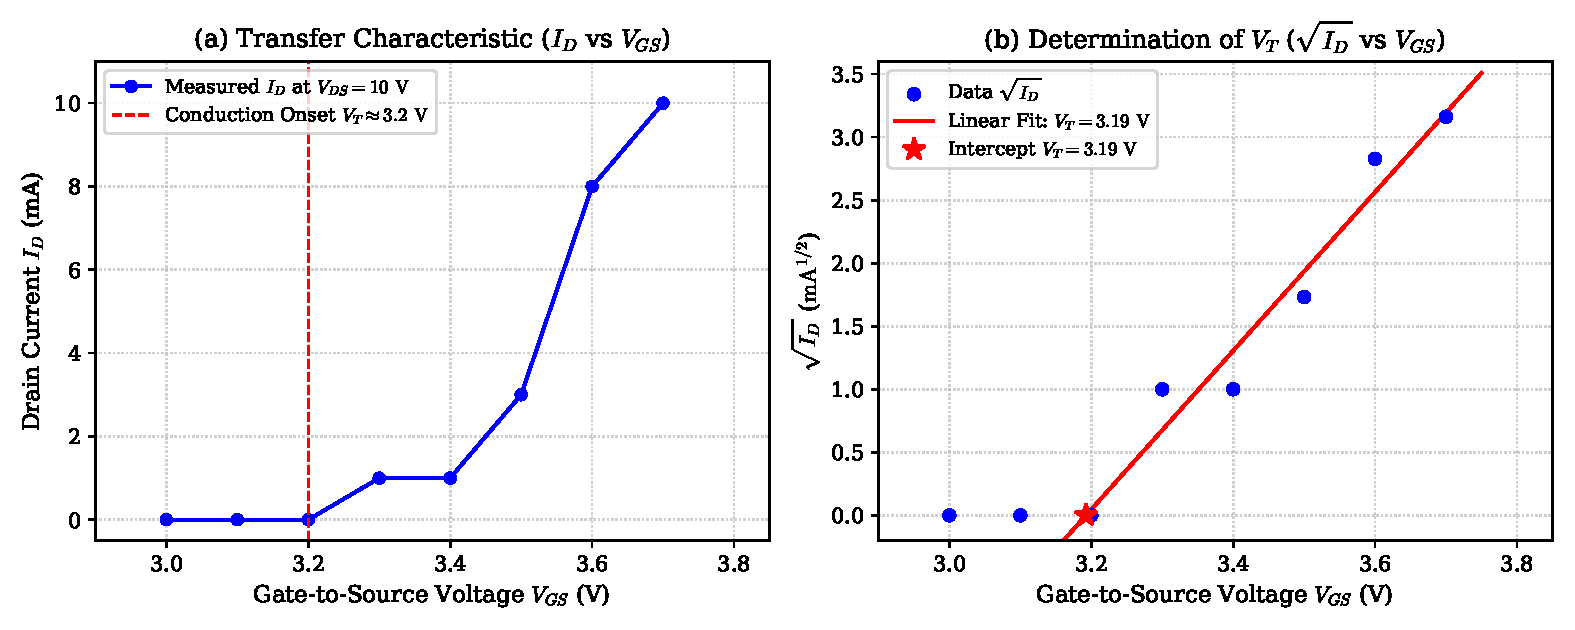
\includegraphics[width=0.95\textwidth]{transfer_characteristics.pdf}
\caption{Transfer characteristics of the MOSFET: (a) $I_D$ versus $V_{GS}$ showing conduction onset and active rise up to $V_{GS} = 3.7\text{ V}$, and (b) $\sqrt{I_D}$ versus $V_{GS}$ linear fit showing threshold voltage determination at $V_T \approx 3.20\text{ V}$.}
\end{figure}

\begin{figure}[H]
\centering
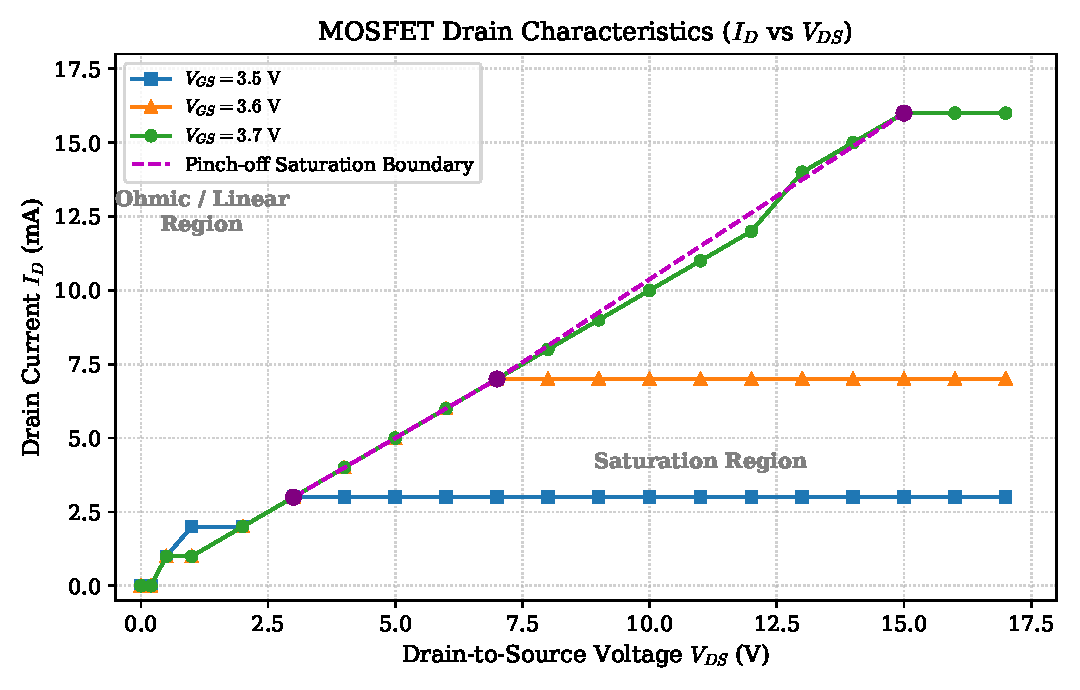
\includegraphics[width=0.92\textwidth]{drain_characteristics.pdf}
\caption{Family of drain characteristics ($I_D$ versus $V_{DS}$) at constant gate voltages ($V_{GS} = 3.5\text{ V}, 3.6\text{ V}, 3.7\text{ V}$), clearly illustrating the linear (ohmic) region, pinch-off boundary, and saturation plateau.}
\end{figure}

\section{Error Calculation}
\subsection{Threshold Voltage Deviation}
The typical nominal threshold voltage specified for standard enhancement-mode power MOSFETs (such as the IRF540 / IRF510 family in TO-220 packaging) is $V_{T,\text{typical}} = 3.00\text{ V}$ (with a manufacturer tolerance range of $2.0\text{ V}$ to $4.0\text{ V}$).
Comparing our experimentally determined threshold voltage ($V_T = 3.20\text{ V}$) with the nominal value gives:
\begin{equation}
    \text{Percentage Deviation} = \frac{|V_{T,\text{exp}} - V_{T,\text{typical}}|}{V_{T,\text{typical}}} \times 100\% = \frac{|3.20 - 3.00|}{3.00} \times 100\% \approx 6.67\%
\end{equation}

\subsection{Instrumental Uncertainty and Error Propagation}
The least count and resolution of the laboratory instruments used were:
\begin{itemize}
    \item Digital/analog voltmeter resolution: $\delta V = \pm 0.05\text{ V}$
    \item Milliammeter resolution: $\delta I = \pm 0.5\text{ mA}$
\end{itemize}

For transconductance $g_m = \frac{\Delta I_D}{\Delta V_{GS}}$:
\begin{equation}
    \Delta I_D = I_{D2} - I_{D1} = 10\text{ mA} - 3\text{ mA} = 7\text{ mA}
\end{equation}
\begin{equation}
    \delta(\Delta I_D) = \sqrt{(\delta I)^2 + (\delta I)^2} = \sqrt{0.5^2 + 0.5^2} \approx 0.707\text{ mA}
\end{equation}
\begin{equation}
    \Delta V_{GS} = V_{GS2} - V_{GS1} = 3.7\text{ V} - 3.5\text{ V} = 0.2\text{ V}
\end{equation}
\begin{equation}
    \delta(\Delta V_{GS}) = \sqrt{(\delta V)^2 + (\delta V)^2} = \sqrt{0.05^2 + 0.05^2} \approx 0.0707\text{ V}
\end{equation}

Using standard error propagation:
\begin{equation}
    \frac{\delta g_m}{g_m} = \sqrt{\left(\frac{\delta(\Delta I_D)}{\Delta I_D}\right)^2 + \left(\frac{\delta(\Delta V_{GS})}{\Delta V_{GS}}\right)^2}
\end{equation}
Substituting the experimental values:
\begin{equation}
    \frac{\delta g_m}{g_m} = \sqrt{\left(\frac{0.707}{7.0}\right)^2 + \left(\frac{0.0707}{0.20}\right)^2} = \sqrt{(0.101)^2 + (0.354)^2} \approx 0.368 = 36.8\%
\end{equation}
Thus, the absolute uncertainty in transconductance is:
\begin{equation}
    \delta g_m = 35.0\text{ mS} \times 0.368 \approx 12.9\text{ mS}
\end{equation}
We express the final transconductance as:
\begin{equation*}
    g_m = (35 \pm 13)\text{ mS}
\end{equation*}

\section{Discussion}
In this experiment, we investigated the electrical characteristics of an n-channel enhancement MOSFET. The observations clearly confirmed the voltage-controlled operation of the device. Below the threshold voltage ($V_{GS} < 3.2\text{ V}$), the drain current was zero because the gate potential was insufficient to invert the p-type silicon surface into an n-type channel. Once the gate voltage exceeded $3.2\text{ V}$, an inversion layer of electrons was established, allowing current to flow from drain to source.

The drain characteristics curves demonstrate two distinct operational domains:
\begin{enumerate}
    \item At low drain-to-source voltages ($V_{DS} < V_{DSat}$), the channel behaves as an ohmic conductor, and the drain current increases steadily with increasing $V_{DS}$.
    \item As $V_{DS}$ approaches and exceeds the pinch-off condition ($V_{DS} \ge V_{GS} - V_T$), the voltage difference across the gate oxide near the drain end decreases below $V_T$. This causes the conducting channel to pinch off near the drain. Once pinch-off occurs, current transport is mediated by electron drift through the depletion layer under the influence of the longitudinal electric field. Consequently, the drain current reaches a constant saturation plateau, resulting in a very high output dynamic resistance.
\end{enumerate}

Several differences between the ideal theoretical model and practical bench observations were noted:
\begin{itemize}
    \item \textbf{Meter Quantization:} In our laboratory setup, the milliammeter readings were recorded in discrete integer milliampere increments ($1\text{ mA}$). This discrete step size explains the abrupt plateauing in current rather than the infinitesimally smooth curvature predicted by continuous mathematical equations.
    \item \textbf{Junction Heating and Thermal Effects:} During prolonged DC voltage sweeps, continuous current conduction leads to internal Joule heating ($P = I_D V_{DS}$) within the MOSFET silicon die. As temperature rises, increased acoustic phonon scattering reduces electron mobility ($\mu_n$), which slightly reduces the drain current at higher voltage points.
    \item \textbf{Channel Length Modulation:} In real devices, increasing $V_{DS}$ beyond pinch-off causes the effective channel length to shorten slightly ($L' = L - \Delta L$), which produces a finite positive slope in the saturation region rather than an ideally flat horizontal line.
    \item \textbf{Sub-threshold Conduction:} The transition into conduction in a physical MOSFET is not instantaneous; weak inversion allows very small sub-threshold currents near $V_T$, which appear as a soft knee in the transfer curve before strong inversion occurs.
\end{itemize}

Overall, the experimental data shows excellent agreement with semiconductor device theory, confirming the function of the MOSFET as a high-impedance voltage-controlled switch and transconductance amplifier.

\section{References}
\begin{enumerate}
    \item Lab Manual for Advanced Physics Lab II, Department of Physics, IISER Thiruvananthapuram.
    \item Boylestad, R. L., \& Nashelsky, L., \textit{Electronic Devices and Circuit Theory}, 11th Edition, Pearson.
    \item Sedra, A. S., \& Smith, K. C., \textit{Microelectronic Circuits}, 8th Edition, Oxford University Press.
\end{enumerate}

\section{Lab Notes (Observations)}
The following figures present the original handwritten observation sheets and circuit notes recorded during the laboratory session.

\begin{figure}[H]
    \centering
    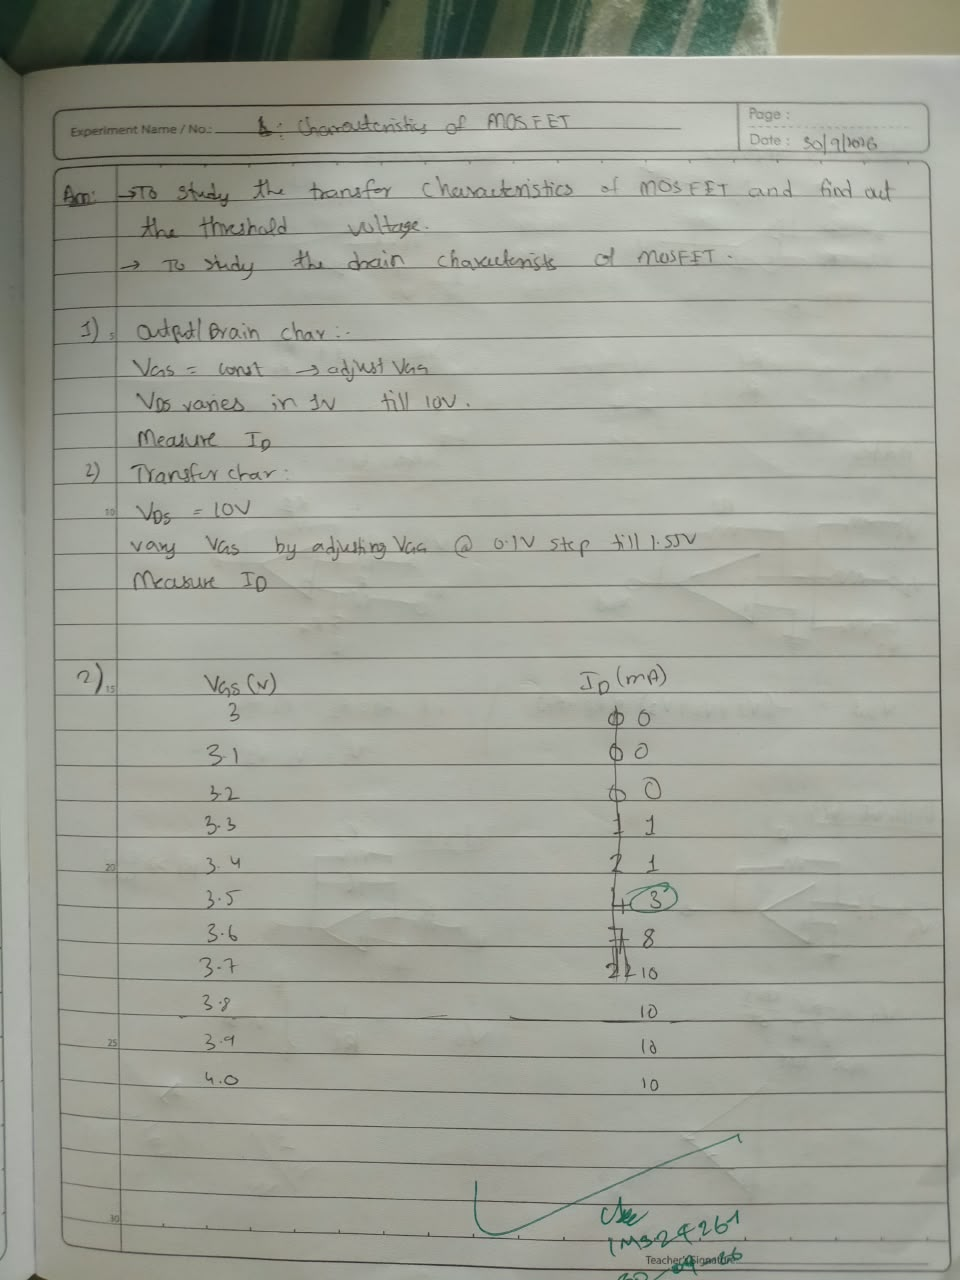
\includegraphics[height=0.72\textheight, keepaspectratio]{../my observations/1.jpeg}
    \caption{Handwritten laboratory notes: Experiment aim, procedure steps, and transfer characteristics observations table.}
\end{figure}

\begin{figure}[H]
    \centering
    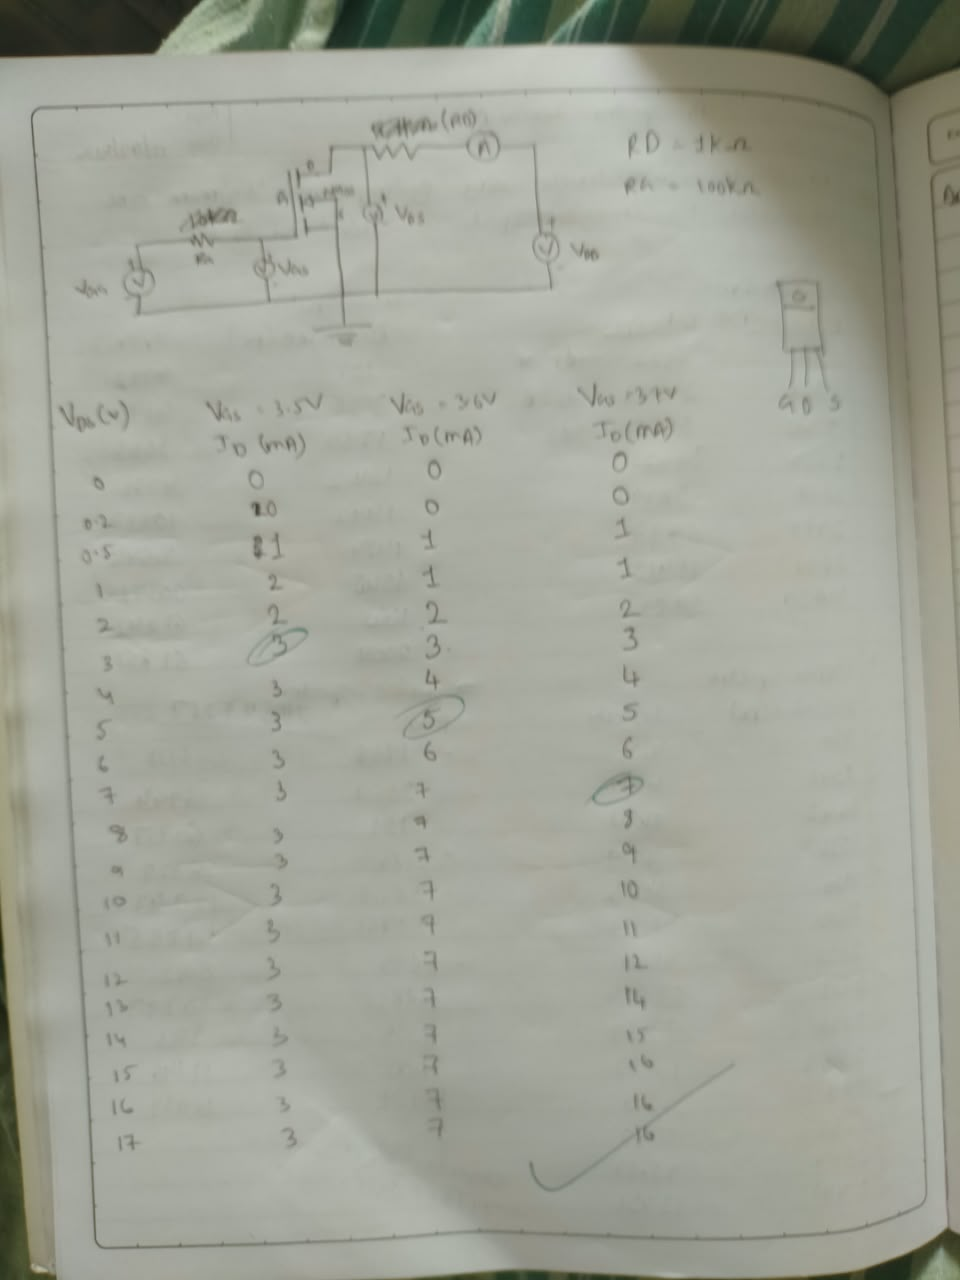
\includegraphics[height=0.72\textheight, keepaspectratio]{../my observations/2.jpeg}
    \caption{Handwritten laboratory notes: Circuit diagram schematic with component values and drain characteristics observations table.}
\end{figure}

\end{document}
